\documentclass[12pt]{article}

\usepackage[french]{babel}
\usepackage{fancyhdr}
\usepackage{amsmath}
\usepackage{amsfonts}
\usepackage[final]{graphicx}
\usepackage{color}
\usepackage{indentfirst}
\usepackage[T1]{fontenc}
\usepackage[justification=centering]{caption}
\usepackage{perpage}
\usepackage{hyperref}
\usepackage{float}
\usepackage[bottom]{footmisc}
\usepackage[a4paper, left=1.2in, right=1.2in, top=1in, bottom=2in]{geometry}
\usepackage{colortbl}
\usepackage{xcolor}
\usepackage[normalem]{ulem}
\useunder{\uline}{\ul}{}

\title{Rapport de projet \\ \textbf{Robot ramasseur de balles de tennis}}
\author{Paul BARBARIN, Mohammed KHERRARZ, Antton CATTARIN}
\date{1A - 2023}

\thispagestyle{plain}

\begin{document}

    \begin{titlepage}

        \begin{figure*}
            \centering
            
\includegraphics{img/enseirb}
        \end{figure*}
        \maketitle

    \end{titlepage}

    \tableofcontents
    \pagebreak
    
    \section{Introduction}

    Le premier objectif de ce projet est de travailler sur différentes méthodes algorithmiques afin de déterminer une solution permettant à un robot de ramasser un ensemble de balles de tennis disposées sur un terrain d'une certaine dimension.

    Son rapprochement avec le cours de théorie des graphes est immédiat, l'ensemble des balles pouvant être représentées comme des sommets. Nous tenterons dans ce rapport d'apporter une solution à ce problème, problème se rapprochant étroitement du problème du voyageur de commerce.
    Quelques spécificités viennent cependant s'ajouter. En effet, le robot est lui-même caractérisé par une vitesse de déplacement ainsi qu'une vitesse de rotation. Les balles étant positionnées à des coordonnées précises, il arrivera dans de nombreux cas où le robot devra effectuer une rotation afin de continuer son parcours.

    Dans un premier temps, nous mettrons en avant et justifierons nos choix de modélisation du problème. Nous discuterons ensuite de la manière d'implémenter ces choix de modélisation en python. Par la suite, nous rentrerons dans la majeure partie du problème. Nous présenterons deux de nos solutions algorithmiques, pour ensuite les comparer et les mettre en confrontation pour la résolution de notre problème. Nous parlerons des inconvénients de chacunes d'elles, ainsi que de leurs avantages.

    \section{Choix de modélisation et implémentation}

    Nous avons choisi d'implémenter le graphe par une matrice d'adjacence de dimension 3. Plus précisément, en considérant qu'il faut prendre en compte la rotation que le robot doit effectuer pour aller d'une balle à une autre en passant par une balle intermédiaire, notre matrice d'ajacence possède les 3 dimensions suivantes :

    \begin{itemize}
        \item Dimension 1 : Sommet précédent (Dernier sommet visité par le robot). Ce sommet présente une très grande importance, car il indique de quel chemin vient le robot et donc par extension son orientation (direction),
        \item Dimension 2 : Sommet courant (Sommet actuellement visité par le robot),
        \item Dimension 3 : Sommet suivant (Sommet suivant à visiter par le robot).
    \end{itemize}

    Cette implémentation du monde en matrice d'adjacence en 3 dimensions permet, en résumé, de représenter le poids, mais également et surtout l'angle entre 3 sommets du graphe, et donc de considérer cela dans le calcul du temps de parcours. Un exemple simple est présenté ci-dessous :

    \begin{figure}[H]
        \centering
        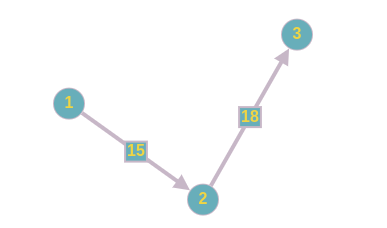
\includegraphics[scale=0.7]{img/example_3dim}
        \caption{3 sommets liés d'un graphe}
        \label{img_3somlinked}
    \end{figure}

    Ici, si $M$ est notre matrice d'adjacence, la valeur $M[1][2][3]$ sera égale au temps que mettra le robot à ramasser la balle 3, en sachant qu'il se situe actuellement sur la balle 2 et qu'il vient de ramasser la balle 1. Cette dernière information nous indique qu'il faut prendre en compte le fait que le robot doit effectuer une rotation de $90$° vers la gauche.

    \section{Deux approches différentes}
    a
    \subsection{Trouver la solution optimale}
    a
    \subsection{Approximer la solution}
    a
    \section{Conclusion}

\end{document}